\documentclass[12pt,a4paper]{article}
\usepackage{indentfirst}
\usepackage[utf8]{inputenc}
\usepackage[T2A]{fontenc}
\usepackage[english,russian]{babel}	% локализация и переносы
\usepackage[left=2cm,right=2cm,top=2cm,bottom=2cm,bindingoffset=0cm]{geometry}
%\usepackage[left=1.5cm,right=2cm,top=2cm,bottom=2cm,bindingoffset=0cm]{geometry}
\usepackage{amsmath,amsfonts,amssymb,amsthm,mathtools} 
\usepackage{wasysym}
\usepackage{multicol}
\usepackage{tikz}
\usepackage{pgf}
\usepackage{pgfplots}
\usepackage{mathrsfs}
\usetikzlibrary{arrows}
\usepackage{wrapfig}
\usepackage{float}
\usepackage{caption}
\usepackage{cmap}
\usepackage{icomma}
\usepackage{hyperref}
%\usepackage[usenames,dvipsnames,svgnames,table,rgb]{xcolor}
\usepackage{xcolor}
\hypersetup{
	unicode=true,
	colorlinks=true,
	linkcolor=red,	   % внутренние
	citecolor=green,   % библиография
	filecolor=magenta, % файлы
	urlcolor=blue      % URL
}

\usepackage{titlesec}
\titlelabel{\thetitle.\:\:}
 
\usepackage{fancyhdr}
\pagestyle{fancy}
\renewcommand{\headrulewidth}{0pt} %default 0.4pt
\renewcommand{\footrulewidth}{0pt}
\lhead{}
\chead{}
\rhead{}
\rfoot{}
%\cfoot{}
\lfoot{}

\theoremstyle{plain}
\newtheorem{theorem}{Теорема}[section]
\newtheorem{proposition}[theorem]{Утверждение}
\newtheorem{problem}{Задача}[section]
\theoremstyle{definition}
\newtheorem{corollary}{Следствие}[theorem]
\theoremstyle{remark}
\newtheorem*{solution}{Решение}
\newtheorem*{Proof}{Доказательство}


\DeclareMathOperator{\poly}{\mathop{poly}}
\DeclareMathOperator{\signum}{\mathop{sign}}
\DeclareMathOperator{\Div}{\mathop{div}}
\DeclareMathOperator{\Rot}{\mathop{rot}}
\DeclareMathOperator{\Grad}{\mathop{grad}}
\newcommand{\parder}[2]{\frac{\partial {#1}}{\partial {#2}}}
\renewcommand{\ge}{\geqslant}
\renewcommand{\le}{\leqslant}
\renewcommand{\phi}{\varphi}
\newcommand{\eps}{\varepsilon}
\renewcommand{\P}{\mathcal{P}}
\newcommand{\NP}{\mathcal{NP}}
\renewcommand{\labelenumii}{\arabic{enumii}.}
\renewcommand{\theenumi}{\large \arabic{enumi}}
\DeclareMathOperator{\per}{\mathop{per}}
\DeclareMathOperator{\FFT}{\mathop{FFT}}
\DeclareMathOperator*{\argmax}{\mathop{argmax}}
\DeclareMathOperator*{\argmin}{\mathop{argmin}}
\renewcommand{\%}[1]{\,\text{mod} \,#1}
\newcommand{\thissection}{} % get current section name
\newcommand{\mysection}[1]{\renewcommand{\thissection}{#1} \section{#1}}
\newcommand{\norm}[1]{\left\lVert#1\right\rVert}
\DeclareMathOperator{\affhull}{\mathop{aff}}
\DeclareMathOperator{\tr}{\mathop{tr}}
\renewcommand{\b}[1]{\mathbf{#1}}
\newcommand{\dkl}[2]{\ensuremath{D_{KL}(#1 \, \lVert \, #2)}}
\newcommand{\T}{\intercal}
\renewcommand{\implies}{\quad \Longrightarrow \quad}

\author{Сысак Михаил Алексеевич}
\title{Отчет о проекте \\ <<Идентификация интернет-пользователей>>}

\begin{document}
	\maketitle
	\section{Описание проекта}
	Идентификация пользователей по их поведению~---~сложная и интересная задача, у которой много применений. В этом проекте решалась задача идентификации пользователей по последовательности сайтов, посещенных ими. В исходном датасете для каждого пользователя имеется csv-файл, в котором последовательно записаны сайты, посещенные пользователем, и время их посещения.
	\section{Первичная обработка и анализ признаков}
	Основной идеей, которая использовалась на протяжении всего проекта, являлось использование мешка слов для хранения обучающей выборки. Недостатком такого подхода является большая размерность данных; достоинством~---~их разреженность, позволившая воспользоваться разреженными матрицами для хранения. 
	
	Обучающие примеры строились следующим образом: из всей последовательности сайтом скользящим окном выделялись последовательности заданной длины, и для каждой такой последовательности создавался объект обучающей выборки. Исследования проводились для размера сессии в $10$ сайтов.
	
	\begin{wrapfigure}{r}{0.4\textwidth}
		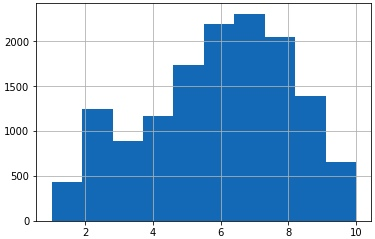
\includegraphics[scale=0.5]{pic1.jpg}
		\caption{Число различных сайтов}\label{pic1}
	\end{wrapfigure}
	На рисунке \ref{pic1} изображена гистограмма числа различных сайтов в сессии. Критерий Шапиро-Уилка уверенно отвергает гипотезу о нормальном распределении этой величины; ясно, что она имеет сложное распределение с двумя пиками.
	
	Для исследования данных были визуально проанализированы различные признаки для выделенных $10$ пользователей. В процессе анализа было замечено, что пользователи принципиально отличаются между собой закономерностями, по которым они посещают различные сайты. Например, кто-то не выходит в интернет в выходные, в то время как другие, наоборот, меньше времени проводят в интернете по будням. У всех пользователей сессии начинаются в разное время дня, по разному распределено и количество сайтов в сессии. Это говорит о том, что по этим данным действительно можно строить идентифицирующую модель.
	\section{Дальнейшее построение признаков}
	По исходным данным был построен ряд признаков, анализ которых был описан в предыдущем разделе. Для каждого пользователя извлекались данные из соответствующей csv-таблицы, и вносились в новый датасет. Были построены следующие признаки:
	\begin{multicols}{2}
		\begin{itemize}
			\item Продолжительность сессии в секундах
			\item Число уникальных сайтов в сессии
			\item Час начала сессии
			\item День недели
			\item Дневное/ночное время
			\item Месяц
			\item Число сайтов в сессии, входящих в топ-$30$ по посещениям
		\end{itemize}
	\end{multicols}
	\section{Сравнение алгоритмов классификации}
	На выборке из $10$ пользователей с длиной сессии $10$ были опробованы различные алгоритмы классификации. Результаты приведены в таблице \ref{table1}.
	\begin{table}[h!]
		\centering
		\begin{tabular}{|c|c|c|}
			\hline
			Алгоритм                & Accuracy на кросс-валидации & Accuracy на отложенной выборке \\ \hline
			KNN                     & 0.565                       & 0.584                          \\ \hline
			Random Forest           & 0.723                       & 0.735                          \\ \hline
			Логистическая регрессия & 0.759                       & 0.775                          \\ \hline
			SVM                     & 0.766                       & 0.782                          \\ \hline
		\end{tabular}
	\caption{Качество различных алгоритмов}\label{table1}
	\end{table}

	Был проведен анализ зависимости качества классификации от длины сессии и ширины окна. Выяснилось, что с ростом длины сессии и уменьшением ширины окна возрастает точность классификации. 
	
	Кроме того, была решена задача классификации одного пользователя против всех остальных, и построена кривая обучения для этой задачи. Она приведена на рисунке \ref{pic2}. Видно, что с увеличением размера выборки увеличивается обобщающая способность алгоритма.
	\begin{figure}[h!]
		\centering
		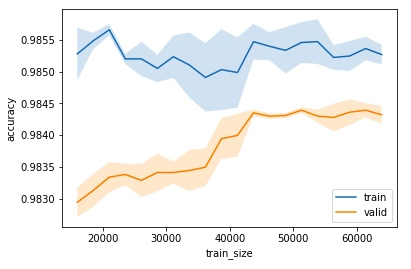
\includegraphics[scale=0.7]{pic2.jpg}
		\caption{Кривые обучения в задаче One-vs-All}\label{pic2}
	\end{figure}
	\section{Дальнейший выбор модели и метрики}
	Была проведена работа с данными соревнования на Kaggle <<Catch me if you can>>. Снова решалась задача идентификации One-vs-All, на этот раз на сильно большей выборке. По этой причине был использован алгоритм SGDClassifier, который хорошо работает с большими объемами данных. В качестве метрики использовался ROC-AUC Score, поскольку он устойчив к несбалансированным выборкам. С помощью GridSearchCV были подобраны параметры алгоритма, побивающие первый бенчмарк. Второй бенчмарк побить не удалось~---~возможно, с этим помогли бы дополнительные признаки. \\
	Для задачи идентификации $400$ пользователей была применена библиотека Vowpal Wabbit. Для сравнения анализировалась также работа SGD и логистической регрессии для этой же задачи. Результаты приведены в таблице \ref{table2}.
	\begin{table}[h!]
		\centering
		\begin{tabular}{|c|c|c|}
			\hline
			Алгоритм                & Точность на отложенной выборке & Время обучения \\ \hline
			Vowpal Wabbit           & 0.345                          & 24.5 s         \\ \hline
			SGDClassifier           & 0.294                          & 24.9 s         \\ \hline
			Логистическая регрессия & 0.363                          & 3min 14s       \\ \hline
		\end{tabular}
	\caption{Сравнение алгоритмов для классификации $400$ пользователей}\label{table2}
	\end{table}

	Из таблицы видно, что VW совмещает в себе лучшее от остальных: он быстро обучается, при этом мало отставая от долгой логистической регрессии.
	\section{Выводы}
	В данном проекте было проведено исследование алгоритмов, метрик и методов для работы с объемными разреженными выборками. Основный вывод состоит в том, что для такого типа задач очень хорого подходит Vowpal Wabbit в силу эффективного распараллеливания и качества, превышающего обычный SGDClassifier. Кроме того, для несбалансированных задач бинарной классификации хорошо подходит метрика ROC-AUC, устойчивая к различным по размеру классам.
	
	Проведенная работа позволяет с уверенностью сказать, что исследованная задача может быть эффективно решена с помощью алгоритмов машинного обучения. Рассмотренные алгоритмы могут применяться для кластеризации пользователей по их предпочтениям в интернете, для ИИ, отличающего владельца аккаунта от взломщика, для идентификации заблокированных пользователей, зашедших с другого IP-адреса, а также для множества других подобных задач. 
\end{document}